\documentclass[11pt,a4paper]{ctexart}

\usepackage[a4paper,margin=2.5cm]{geometry}
\usepackage{graphicx}
\usepackage{float}
\usepackage{booktabs}
\usepackage{longtable}
\usepackage{array}
\usepackage{amsmath,amssymb}
\usepackage{hyperref}
\usepackage{xcolor}
\usepackage{fancyvrb}
\usepackage{caption}

\hypersetup{
  colorlinks=true,
  linkcolor=blue,
  urlcolor=blue
}

\title{软件设计与编程实践实验报告}
\author{陶樞臣 2024050524}
\date{2026年4月21日}

\begin{document}

\maketitle

\begin{abstract}
本次实验完成了一个基于 Web 的交互式信号时域与频域分析工具，并围绕带高斯白噪声的正弦信号展开测试与验证。报告从实验目的、算法理论、实验环境、系统实现、测试过程以及结果分析几个方面，对时域统计分析、FFT 频谱分析、预处理方法以及系统的交互式实现进行了整理与说明。
\end{abstract}

\section{实验目的}

本次实验是《软件设计与编程实践》课程的期中实践环节，旨在通过完整的工具开发过程，完成以下目标：

\begin{enumerate}
  \item 掌握数字信号处理中时域分析与频域分析的基本原理，理解信号从时域到频域转换的内在逻辑。
  \item 深入理解快速傅里叶变换（FFT）算法的原理与实现方式，掌握其在信号频谱分析中的应用。
  \item 掌握前端 Web 技术的应用，实现交互式的数据处理与可视化功能，理解事件驱动编程的特点。
  \item 培养从数据导入、预处理、核心算法处理到结果可视化的完整工程化开发能力，建立模块化的编程思维。
  \item 能够对带噪声的实际采样信号进行有效的特征提取与分析，验证算法在实际场景中的有效性。
\end{enumerate}

\section{算法理论分析及仿真}

\subsection{时域分析原理}

时域分析是最基础的信号分析方法，它直接对采样得到的信号序列进行分析，描述信号幅度随时间的变化特征。在本次实验中，主要计算了以下时域统计特征：

\begin{itemize}
  \item \textbf{峰值（Peak）}：信号的最大值，描述信号的最大正向幅度。
  \item \textbf{谷值（Valley）}：信号的最小值，描述信号的最大负向幅度。
  \item \textbf{峰峰值（Peak-to-Peak）}：峰值与谷值的差值，描述信号的整体波动范围。
  \item \textbf{均值（Mean）}：信号的平均值，描述信号的直流偏移量。
\end{itemize}

这些统计量可以直观反映信号的幅值特征，是信号分析中的基础指标。

\subsection{频域分析与 FFT 原理}

频域分析将信号从时间域转换到频率域，从而直观地查看信号的频率组成，提取信号的频率特征。其核心是傅里叶变换，它可以将任意时域信号分解为不同频率的正弦信号叠加。

离散傅里叶变换（DFT）的定义为
\[
X[k] = \sum_{n=0}^{N-1} x[n] e^{-j 2\pi kn/N}, \quad k = 0, 1, \ldots, N-1.
\]

直接计算 DFT 的时间复杂度为 $O(N^2)$。当信号长度较大时，计算效率较低。快速傅里叶变换（FFT）是 DFT 的高效实现，通过利用旋转因子的对称性和周期性，将计算复杂度降低为 $O(N\log N)$，极大提升了频谱分析效率。

对于实信号，FFT 结果具有共轭对称性，因此只需取前半部分结果即可构成单边幅度谱。这样既能保留主要信息，也能使频谱结果更加直观。

\subsection{预处理原理}

为了提升频谱分析效果，实验中加入了如下预处理步骤：

\begin{enumerate}
  \item \textbf{去直流处理}：移除信号均值，减弱直流分量对频谱结果的影响，避免低频区域被直流偏置掩盖。
  \item \textbf{加窗处理}：对信号施加窗函数，减少频谱泄漏，提升频谱分析精度，并支持根据分析场景选择不同窗函数。
  \item \textbf{补零处理}：将信号长度补齐到 2 的整数次幂，以提高 FFT 计算效率。
\end{enumerate}

\subsection{仿真分析}

本次实验使用的仿真测试信号为带高斯白噪声的 2\,kHz 正弦波，其表达式为
\[
x(t) = A \sin(2\pi f_0 t) + n(t).
\]

其中，$A = 1.2$ 为信号幅值，$f_0 = 2000\,\text{Hz}$ 为信号基频，$n(t)$ 为高斯白噪声。

采样参数设置为：采样率 $F_s = 1000000\,\text{Hz}$，采样点数 $N = 4096$。根据采样定理，该采样率远高于信号最高频率，奈奎斯特频率为 500\,kHz，因此不会发生频率混叠。频率分辨率为
\[
\Delta f = \frac{F_s}{N} = 244.140625\,\text{Hz}.
\]

仿真结果表明，时域波形为带噪声的正弦波，频域主峰出现在 2\,kHz 附近，其余噪声成分均匀分布在整个频域范围内，符合理论预期。

\section{实验环境}

\subsection{硬件环境}

\begin{itemize}
  \item 处理器：Intel Core i7-13900HX CPU @ 2.90GHz
  \item 内存：32GB DDR5 2666MHz
  \item 存储：1TB NVMe SSD
\end{itemize}

\subsection{软件环境}

\begin{itemize}
  \item 操作系统：Windows 11 企业版
  \item 浏览器：Google Chrome 124.0.6367.60（64 位）
  \item 编程环境：HTML5、JavaScript ES6
  \item 依赖库：Chart.js 4.3.0、fft.js 0.3.0
\end{itemize}

\section{实验过程与分析}

\subsection{功能模块划分}

根据程序的功能需求与流程设计，整个系统划分为 4 个独立功能模块：

\begin{enumerate}
  \item \textbf{页面初始化与主控制模块}：负责页面加载后的初始化、图表实例创建、事件绑定以及程序状态管理。
  \item \textbf{CSV 数据导入与预处理模块}：负责读取本地 CSV 文件，解析单列或双列数据，并自动生成或识别时间向量与采样率。
  \item \textbf{信号分析核心模块}：执行去直流、时域特征计算、加窗、补零及 FFT 运算，并生成单边幅度谱。
  \item \textbf{可视化与交互模块}：负责时域图、频域图以及统计面板的展示与更新，并响应坐标范围、窗函数、采样率等交互操作。
\end{enumerate}

\subsection{程序操作流程}

整个程序采用事件驱动运行模式。页面加载完成后先完成初始化，再进入等待用户操作的循环。用户导入 CSV 文件、切换窗函数、勾选去直流选项或修改采样率时，程序会重新进行分析；若仅调整图表显示范围，则只更新图表显示，不重新执行完整分析流程。

\begin{figure}[H]
  \centering
  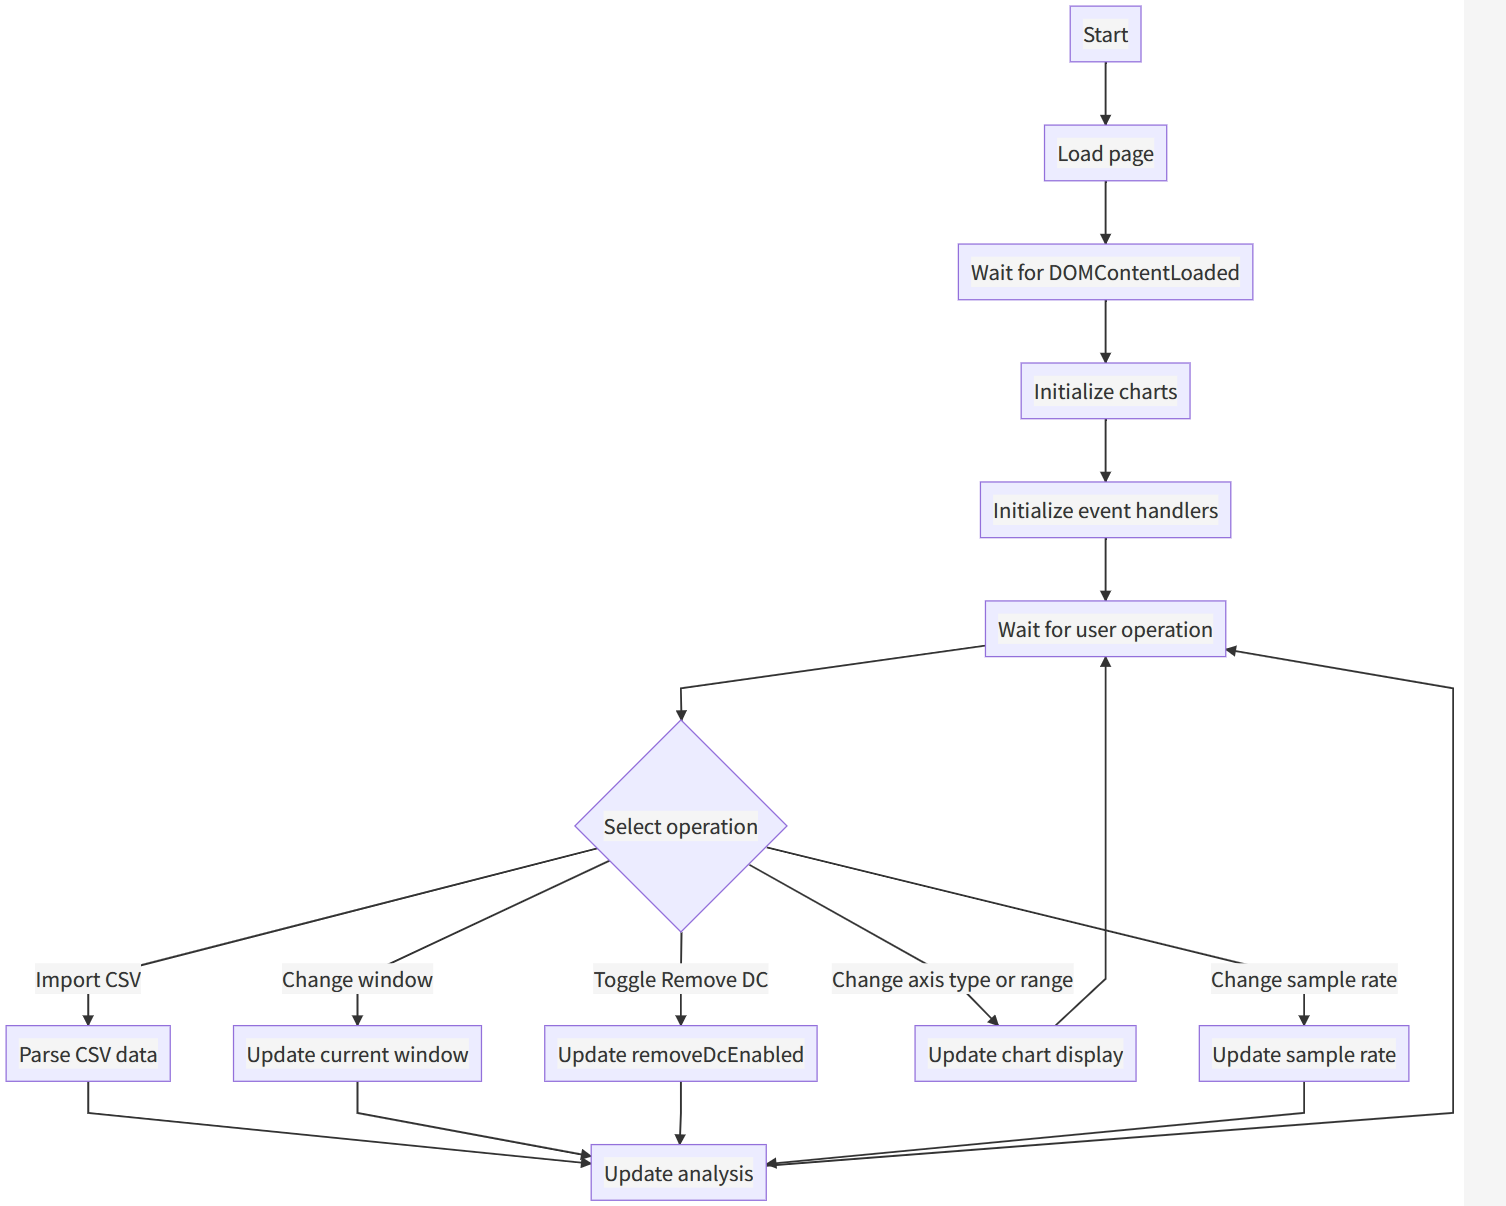
\includegraphics[width=0.78\textwidth]{image/FlowChart4-21-3.png}
  \caption{程序总体操作流程图}
\end{figure}

信号导入与解析流程包括打开文件选择器、读取文本、逐行解析、判断数据列格式、补全时间向量、计算采样率，并在导入成功后触发完整分析流程。

\begin{Verbatim}[frame=single,fontsize=\small]
BEGIN
    ENTER updateAnalysis
    IF no signal data THEN
        RETURN
    END IF
    COPY original signal
    IF DC removal enabled THEN
        REMOVE signal mean
    END IF
    CALCULATE peak, valley, peak-to-peak, mean, sample rate, frequency resolution
    UPDATE statistics panel
    UPDATE time-domain chart
    APPLY selected window function
    PAD data to next power of two
    EXECUTE FFT
    CALCULATE single-sided spectrum amplitude
    UPDATE frequency-domain chart
END
\end{Verbatim}

\subsection{关键代码设计与分析}

\subsubsection{CSV 数据解析代码}

该部分代码用于初始化图表并为后续的数据导入与显示提供基础支持。程序首先创建时域图与频域图实例，分别配置横纵坐标、线条样式与提示信息，以便在导入数据后实时更新显示。

\begin{Verbatim}[frame=single,fontsize=\small]
function initCharts() {
    if (typeof Chart === "undefined") {
        showStatus("Loading Failed...", true);
        return;
    }

    const timeCtx = document.getElementById("time-domain-chart").getContext("2d");
    timeDomainChart = new Chart(timeCtx, {
        type: "line",
        data: {
            labels: [],
            datasets: [{
                label: "Time Domain",
                data: [],
                borderColor: "rgb(75, 192, 192)",
                tension: 0.1,
                pointRadius: 0,
                borderWidth: 1.5
            }]
        }
    });
}
\end{Verbatim}

\subsubsection{信号分析核心代码}

核心分析代码负责完成信号预处理、统计量计算以及 FFT 频谱分析。程序会先复制原始信号，在需要时去除直流分量，再计算峰值、谷值、峰峰值、均值与频率分辨率，随后对信号进行加窗和补零，并执行 FFT 计算，最终得到单边幅度谱并更新频域图表。

\begin{Verbatim}[frame=single,fontsize=\small]
function updateAnalysis() {
    if (!originalAmplitude || originalAmplitude.length === 0) return;

    let signal = [...originalAmplitude];

    if (removeDcEnabled) {
        const mean = signal.reduce((a, b) => a + b, 0) / signal.length;
        signal = signal.map(v => v - mean);
    }

    const peak = Math.max(...signal);
    const valley = Math.min(...signal);
    const peakToPeak = peak - valley;
    const mean = signal.reduce((a, b) => a + b, 0) / signal.length;
    const freqResolution = sampleRate / signal.length;

    updateStats(peak, valley, peakToPeak, mean, sampleRate, freqResolution);
    updateTimeDomainChart(originalTime, signal);

    const window = getWindowFunction(signal.length);
    signal = signal.map((v, i) => v * window[i]);

    const nextPowerOf2 = 1 << Math.ceil(Math.log2(signal.length));
    const padded = [...signal, ...new Array(nextPowerOf2 - signal.length).fill(0)];
    const fftResult = fft(padded);

    const spectrum = [];
    const freqAxis = [];
    for (let i = 0; i < nextPowerOf2 / 2; i++) {
        const re = fftResult[i].re;
        const im = fftResult[i].im;
        const amplitude = Math.sqrt(re * re + im * im) * 2 / nextPowerOf2;
        spectrum.push(amplitude);
        freqAxis.push(i * sampleRate / nextPowerOf2);
    }

    updateFrequencyDomainChart(freqAxis, spectrum);
}
\end{Verbatim}

\subsection{测试参数设计}

为了验证程序正确性，实验选取带噪声的正弦信号作为测试输入。测试参数如表~\ref{tab:test-params} 所示。

\begin{table}[H]
  \centering
  \caption{测试参数设计}
  \label{tab:test-params}
  \begin{tabular}{>{\raggedright\arraybackslash}p{3.2cm} >{\raggedright\arraybackslash}p{4.0cm} >{\raggedright\arraybackslash}p{6.0cm}}
    \toprule
    参数项 & 参数值 & 说明 \\
    \midrule
    测试文件 & \texttt{sine\_wave\_4096.csv} & 包含采样信号的 CSV 文件 \\
    采样点数 & 4096 & 信号的总采样数 \\
    采样率 & 1000000 Hz & 信号的采样频率 \\
    信号基频 & 2000 Hz & 正弦波的基础频率 \\
    信号幅值 & 1.2 & 正弦波的标称幅值 \\
    噪声类型 & 高斯白噪声 & 叠加的噪声类型 \\
    信噪比 & 约 15 dB & 测试中设定的信噪比 \\
    预处理选项 & 未开启去直流，使用寒凝窗函数 & 本次测试使用的默认预处理参数 \\
    \bottomrule
  \end{tabular}
\end{table}

\subsection{测试与调试}

在测试过程中，针对程序各个功能模块进行了逐项验证与调试：

\begin{enumerate}
  \item \textbf{数据导入测试}：导入测试 CSV 文件后，程序成功识别 4096 个采样点，正确解析幅值数据，并依据采样率生成对应时间向量，导入过程稳定。
  \item \textbf{时域分析测试}：程序能够正确计算峰值、谷值、峰峰值与均值等统计量，验证了时域分析模块的基本正确性。
  \item \textbf{频域分析测试}：程序成功执行 FFT，并给出单边幅度谱，频率分辨率计算结果与理论值
  \[
  \frac{10^6}{4096} = 244.140625\,\text{Hz}
  \]
  完全一致。
  \item \textbf{交互功能测试}：调整坐标范围、切换窗函数等交互操作均能快速响应。仅修改显示范围时不会触发重复分析，切换窗函数后可正确刷新频谱结果。
  \item \textbf{边界情况调试}：针对空文件、格式错误文件等异常情况进行了验证，程序能够正确处理异常输入，避免崩溃，提高系统稳健性。
\end{enumerate}

\section{实验结果显示与验证}

本次实验的程序运行结果如图所示。

\begin{figure}[H]
  \centering
  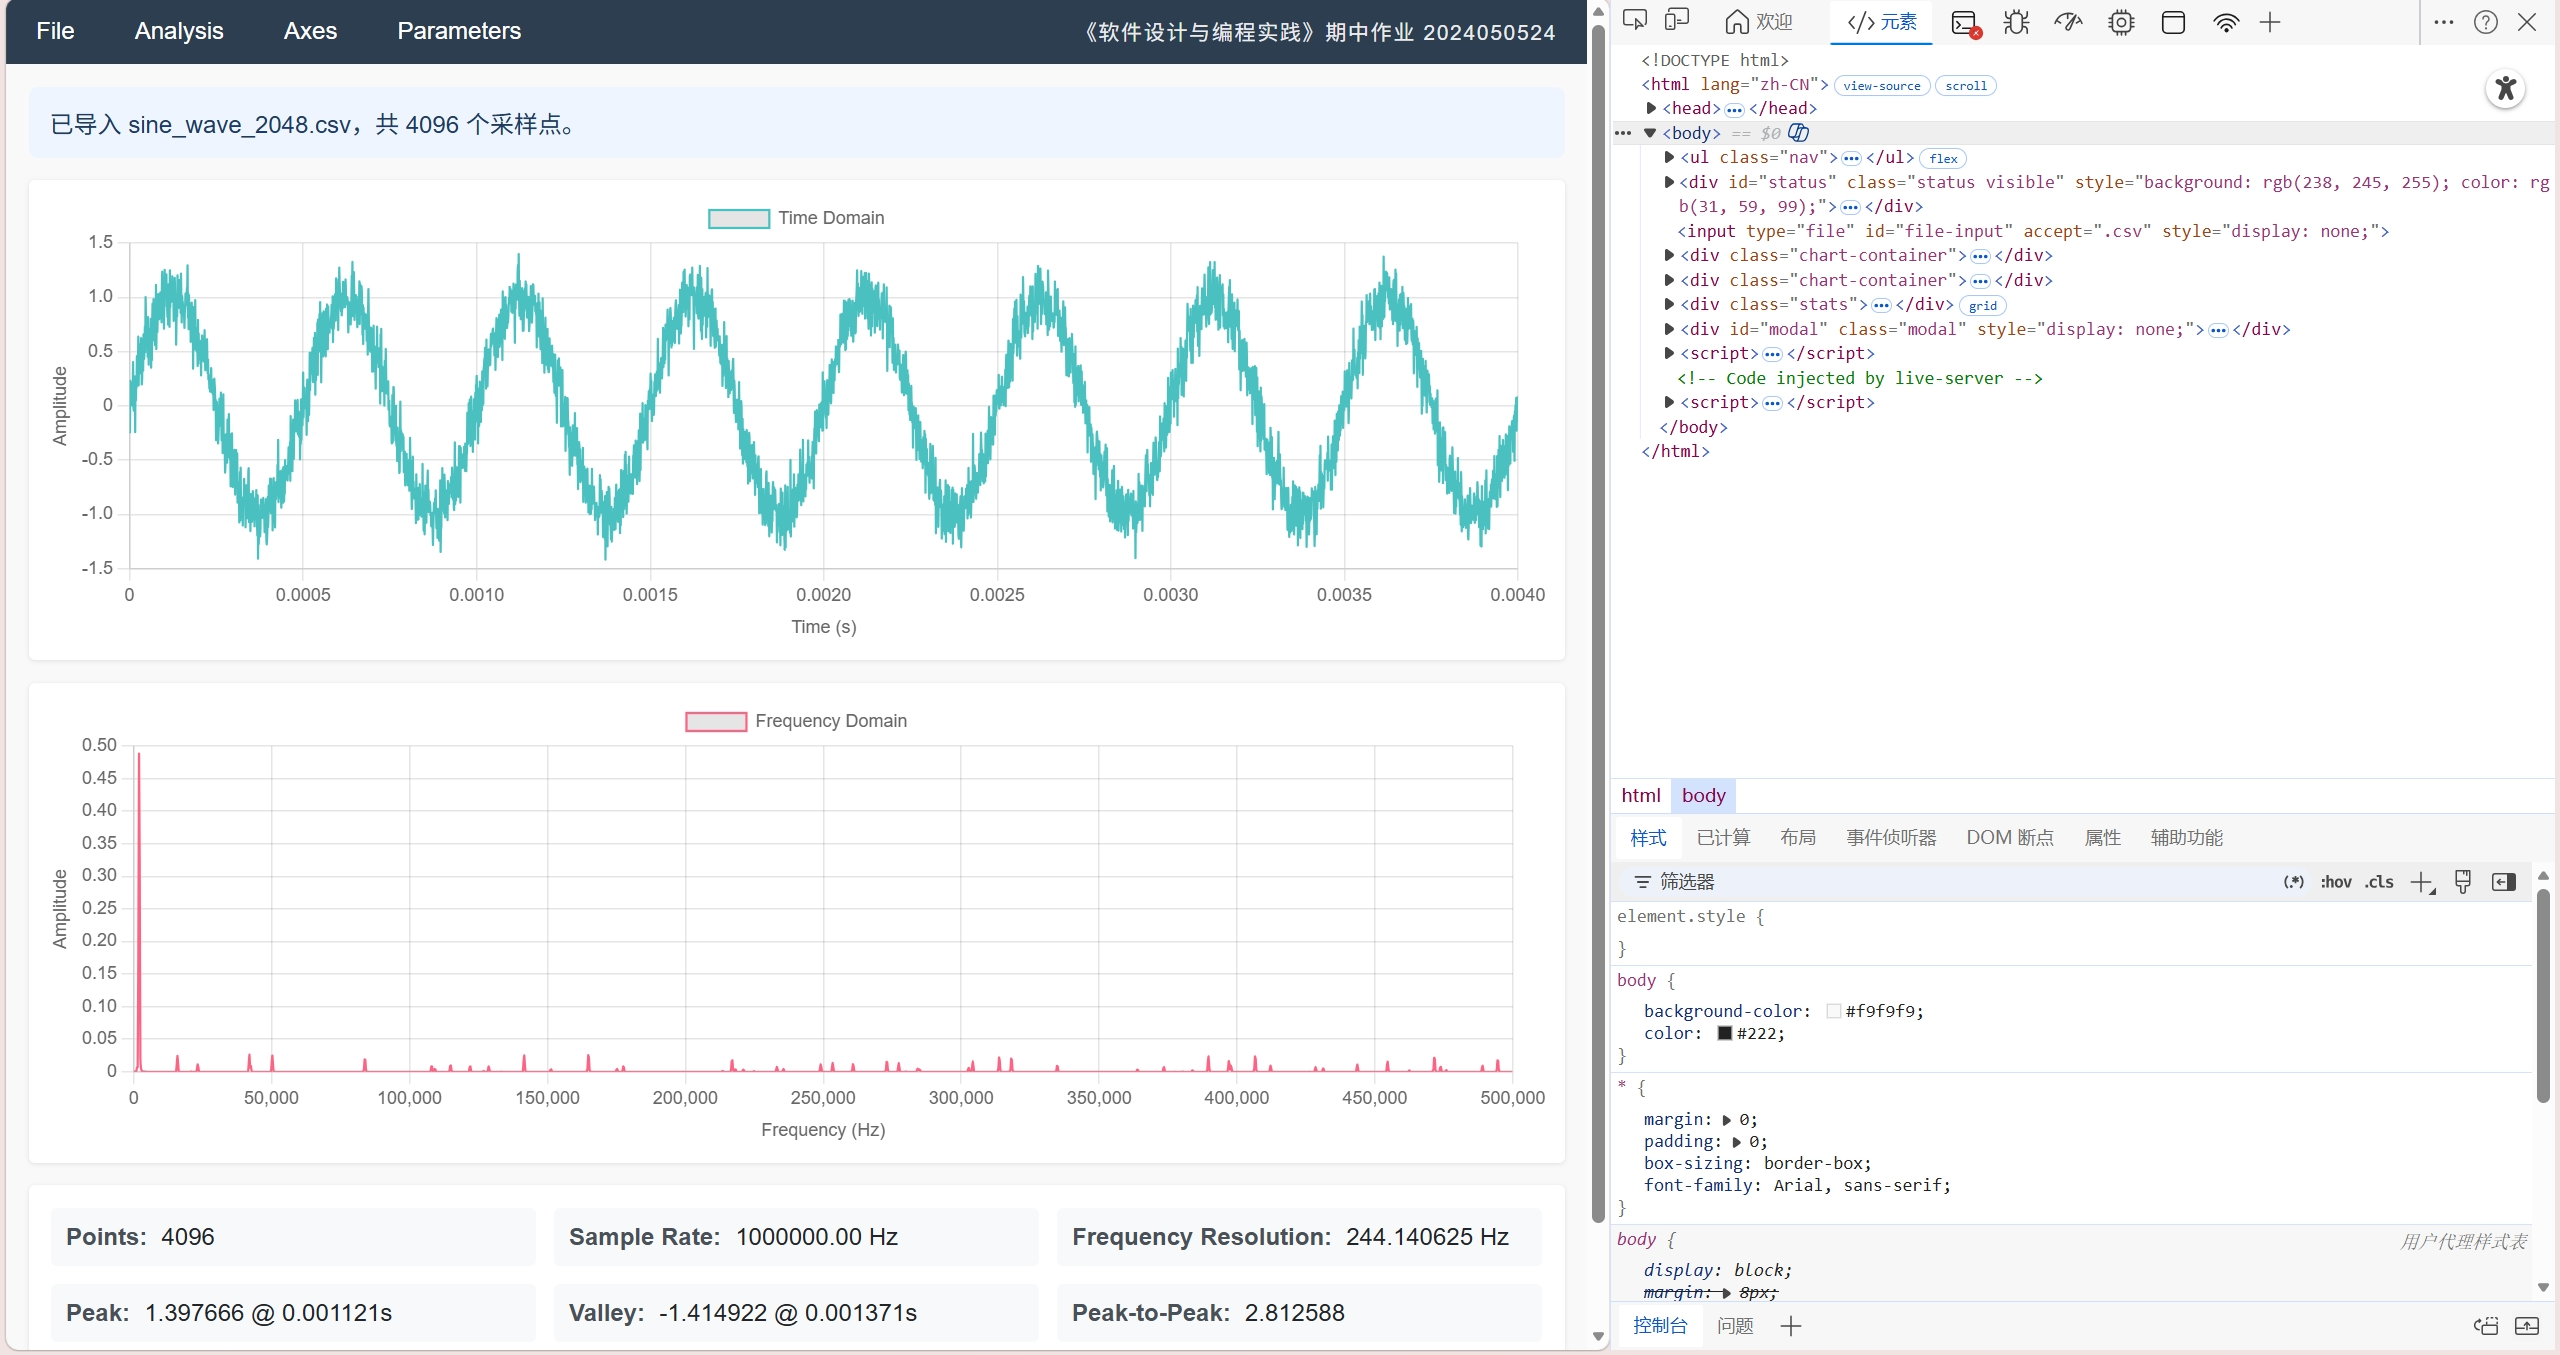
\includegraphics[width=0.82\textwidth]{image/4-21-1.png}
  \caption{程序运行结果总览}
\end{figure}

\begin{figure}[H]
  \centering
  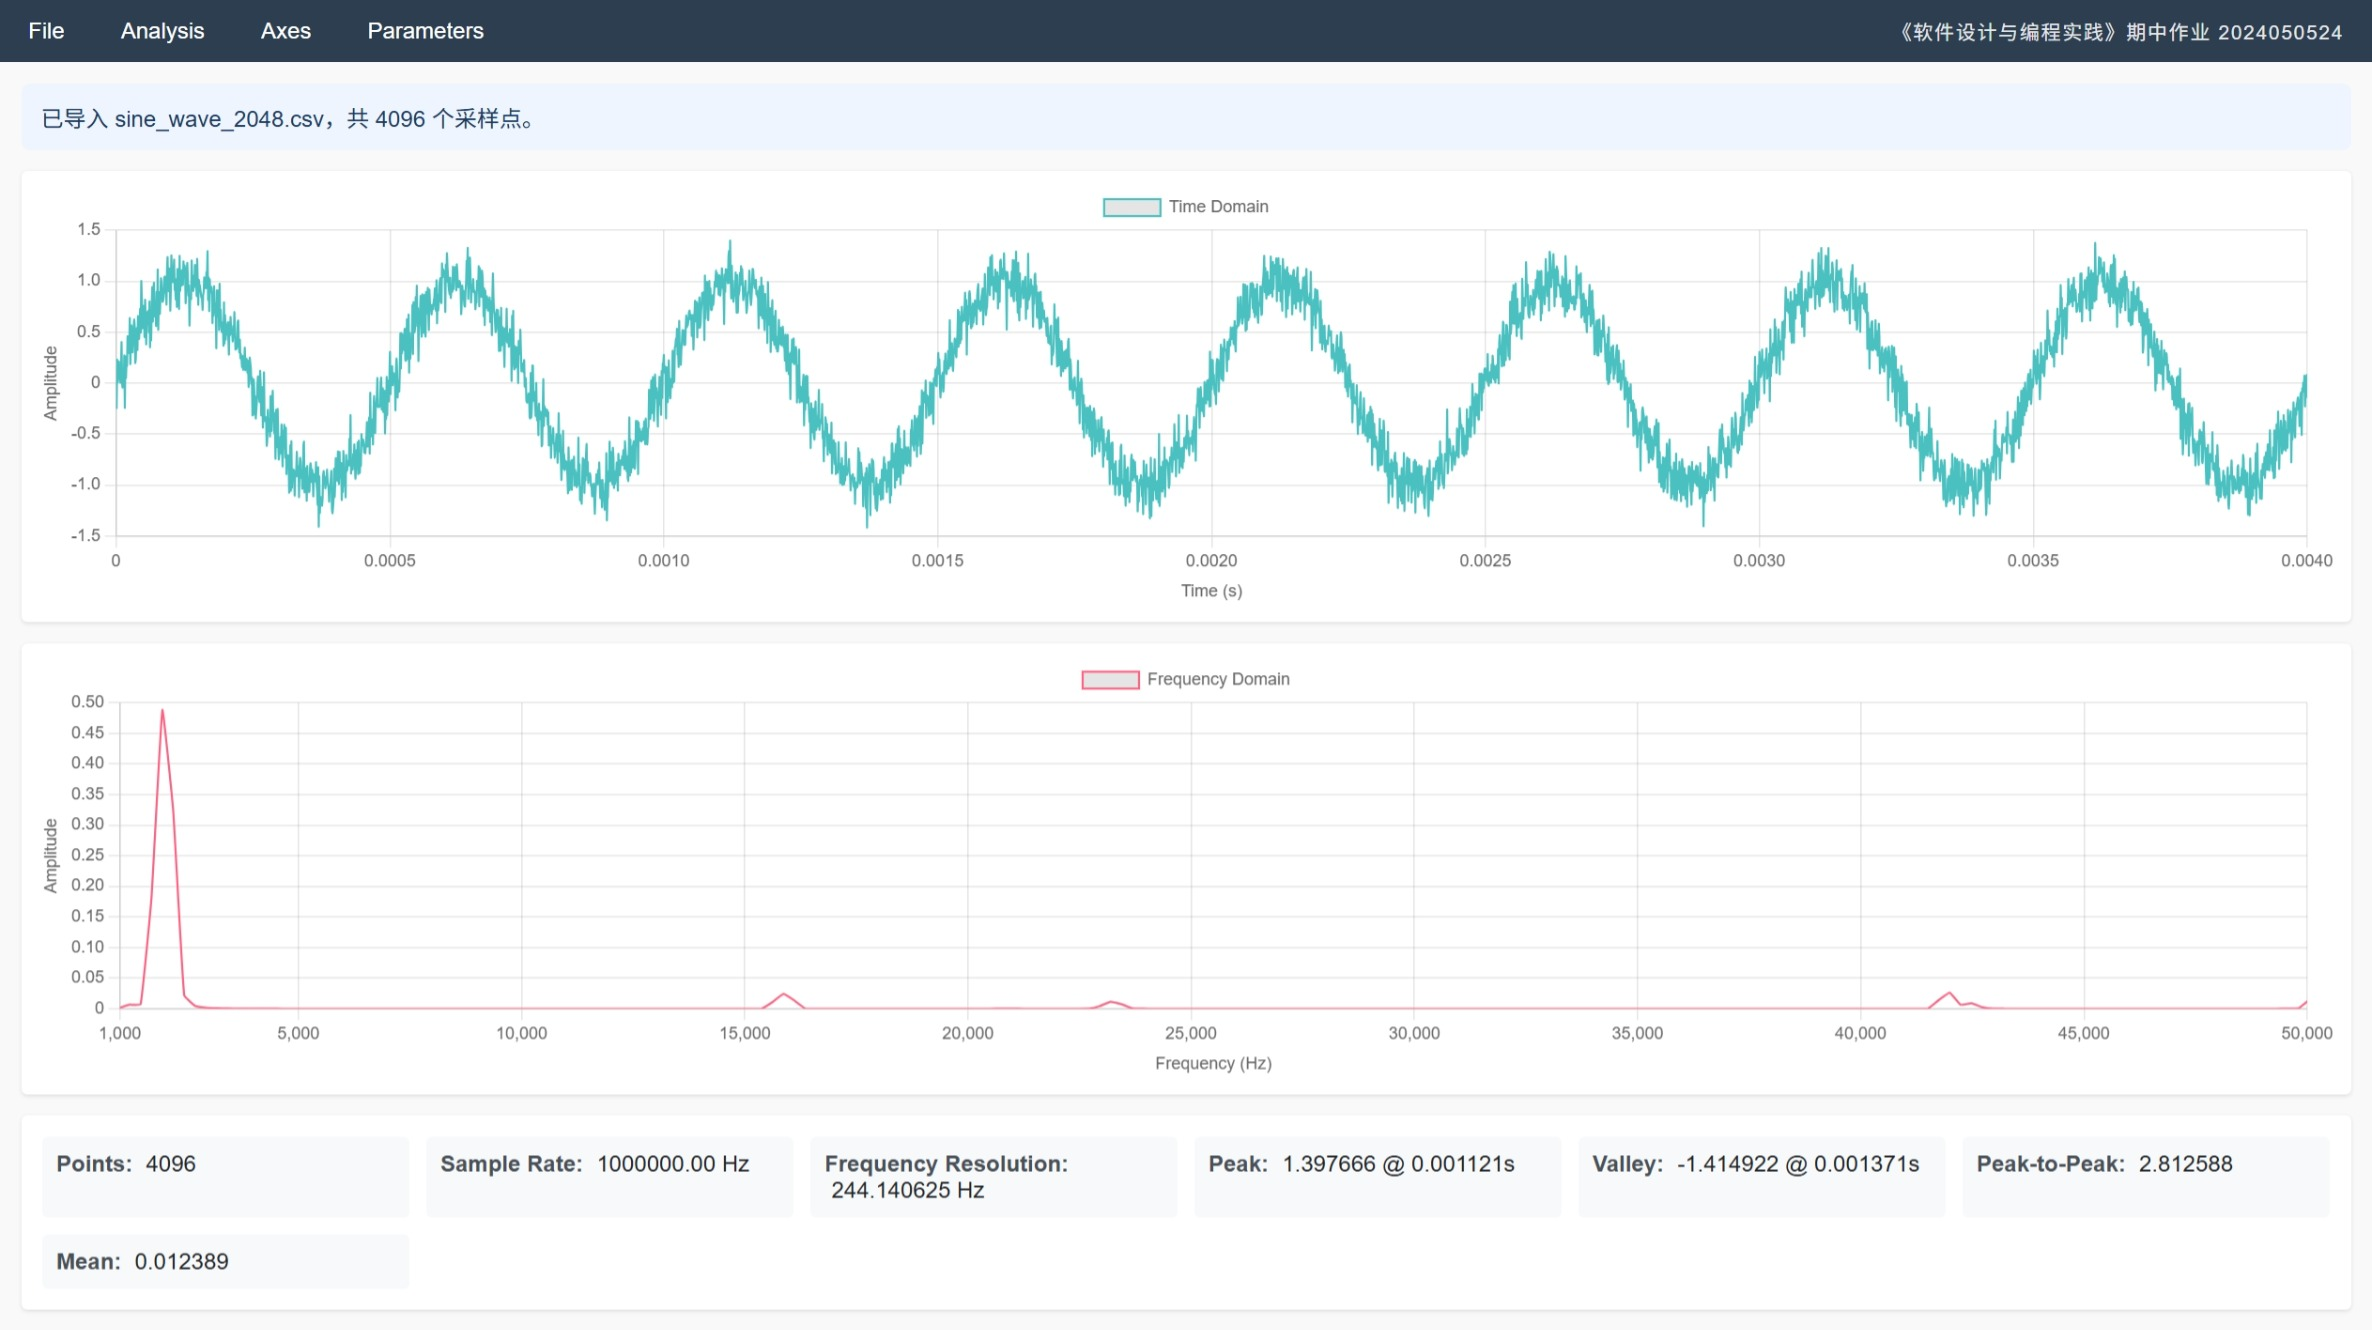
\includegraphics[width=0.82\textwidth]{image/4-21-1.jpeg}
  \caption{时域与频域分析显示}
\end{figure}

\begin{figure}[H]
  \centering
  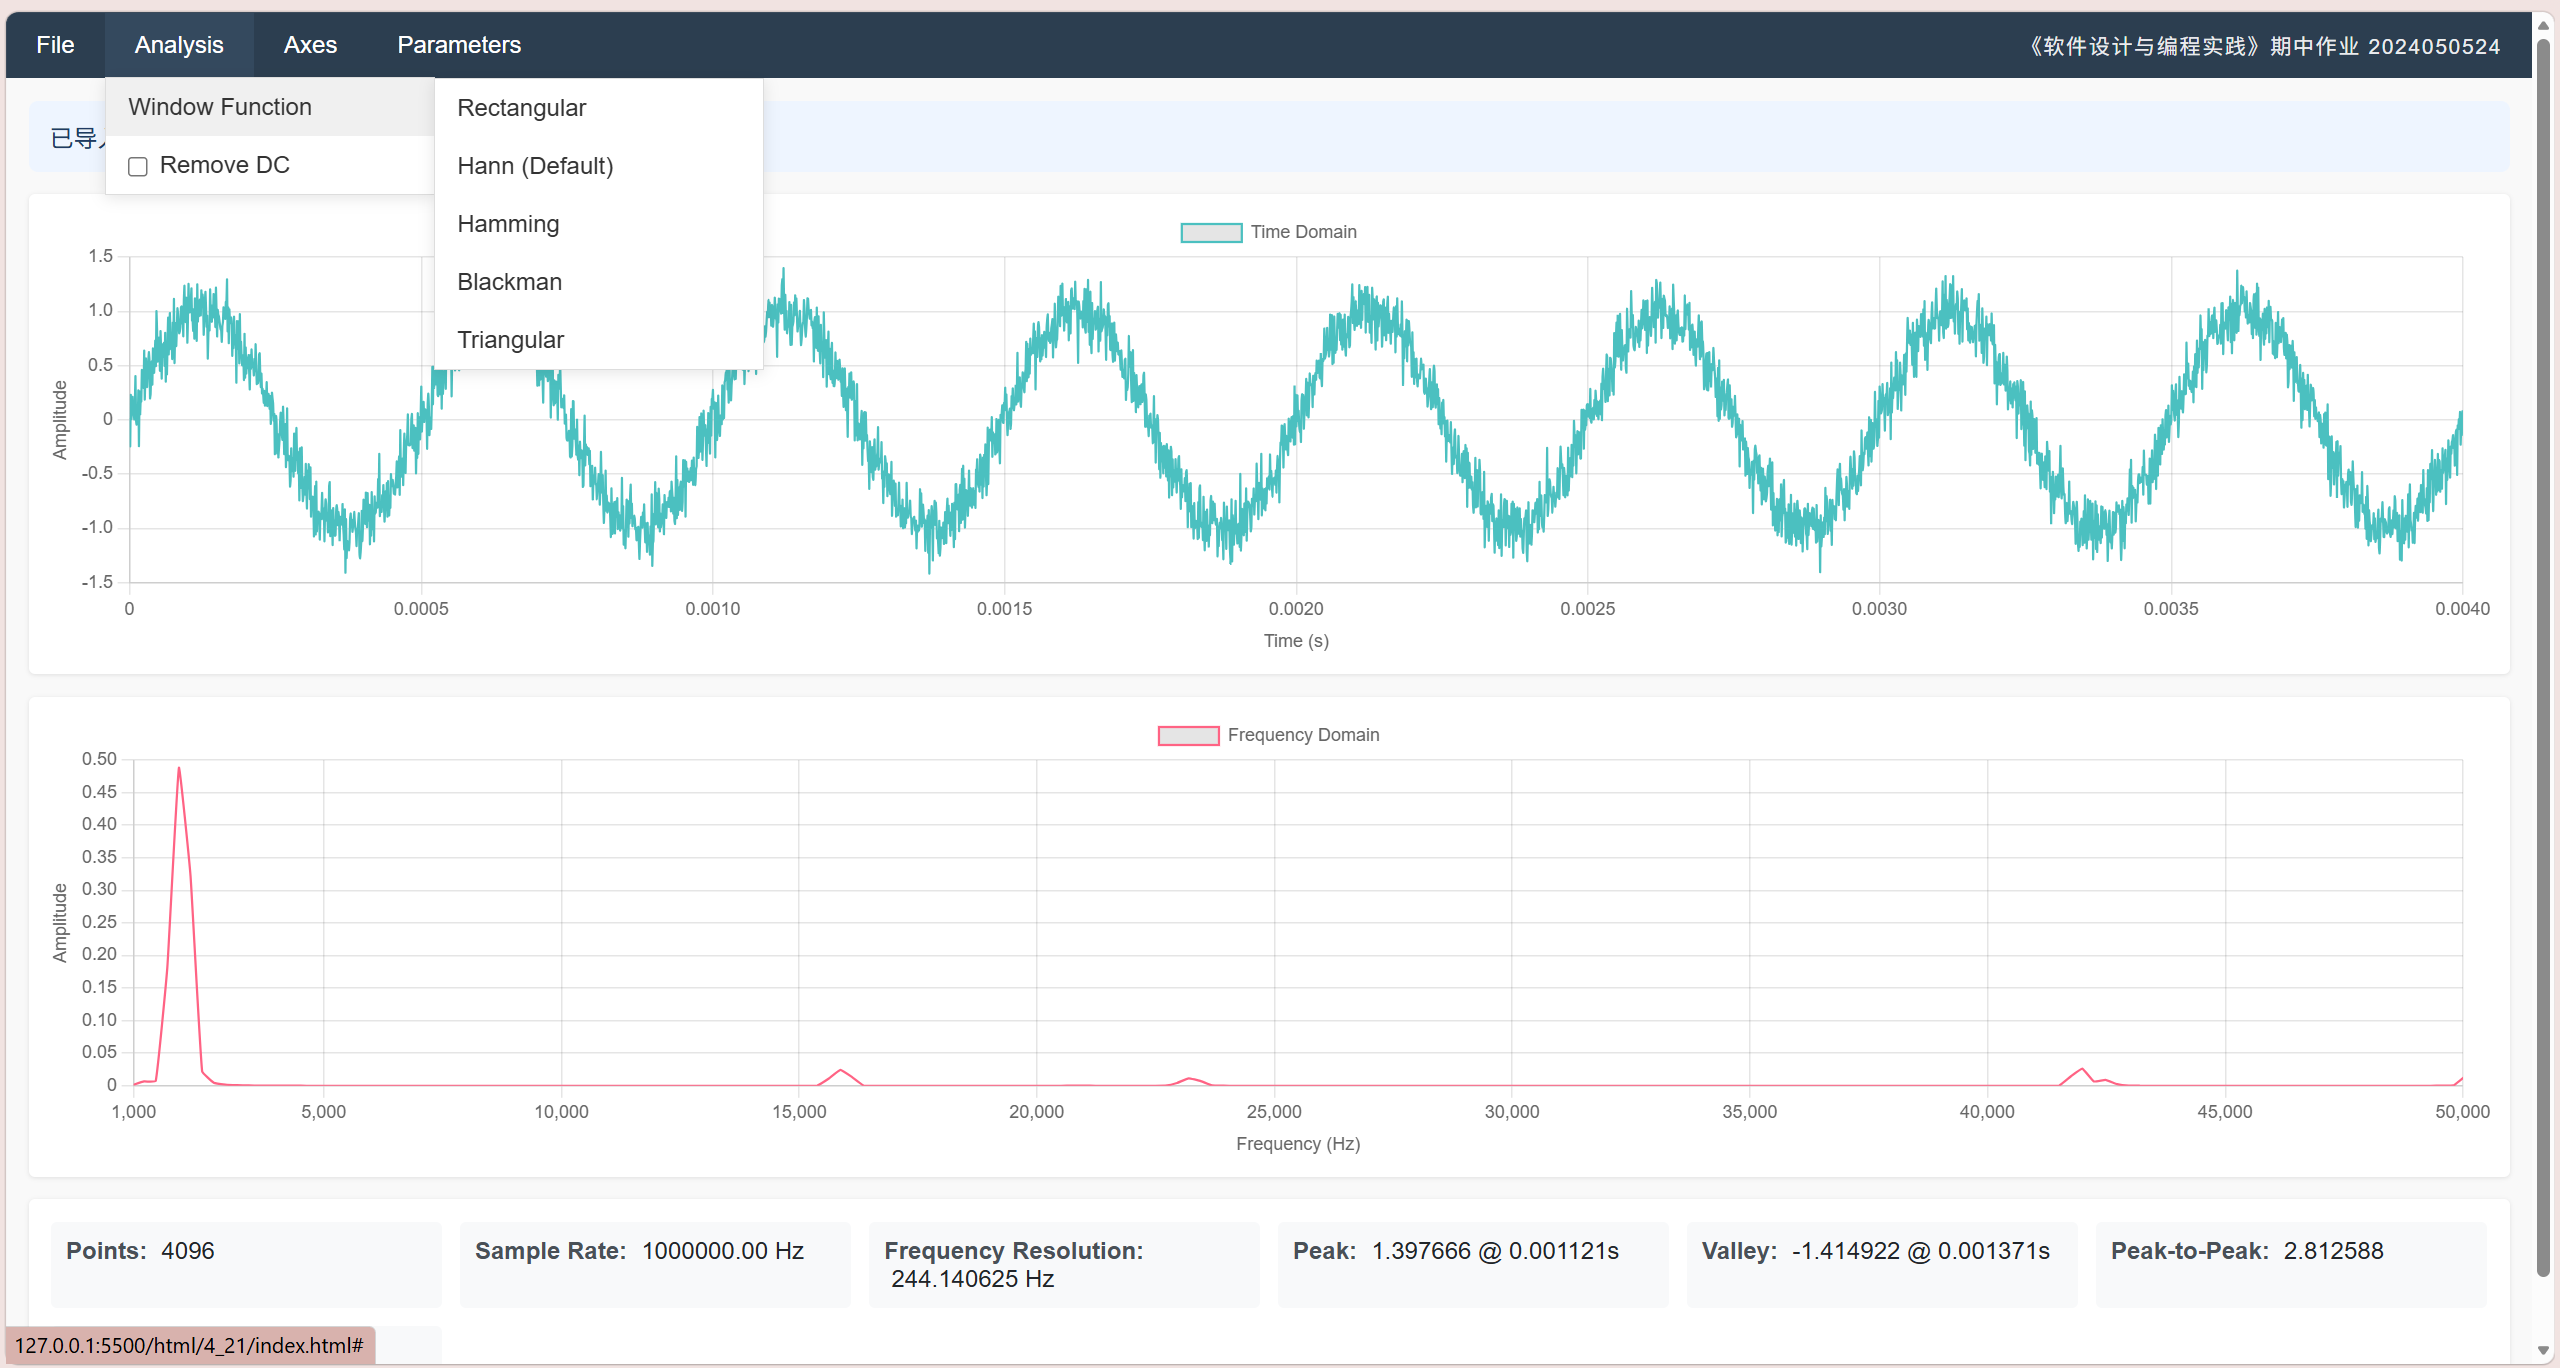
\includegraphics[width=0.82\textwidth]{image/4-21-2.png}
  \caption{交互功能测试结果}
\end{figure}

\subsection{结果分析}

从运行结果中可以得到如下信息：

\begin{enumerate}
  \item \textbf{时域波形分析}：时域波形图显示了带噪声的 2\,kHz 正弦信号。在 0--0.004\,s 的时间范围内，信号完成了 8 个完整周期，与 2000\,Hz 的基频相符。由于叠加了高斯噪声，波形存在一定毛刺，但整体周期性明显。
  \item \textbf{频域频谱分析}：频谱图中主峰出现在 2\,kHz 附近。考虑到频率分辨率为 244.140625\,Hz，主峰位置与理论值一致，其余较小峰值主要来源于高斯白噪声成分。
  \item \textbf{统计参数验证}：程序给出的统计量与理论预期一致。峰值和谷值略高于和低于理想值，说明噪声影响真实存在；均值接近 0，说明直流偏移较小。
\end{enumerate}

\begin{table}[H]
  \centering
  \caption{统计参数对比}
  \begin{tabular}{>{\raggedright\arraybackslash}p{2.7cm} >{\centering\arraybackslash}p{3.2cm} >{\centering\arraybackslash}p{3.0cm} >{\raggedright\arraybackslash}p{5.0cm}}
    \toprule
    参数项 & 程序计算值 & 理论预期值 & 对比结果 \\
    \midrule
    采样点数 & 4096 & 4096 & 完全一致 \\
    采样率 & 1000000.00 Hz & 1000000.00 Hz & 完全一致 \\
    频率分辨率 & 244.140625 Hz & 244.140625 Hz & 完全一致 \\
    峰值 & 1.397666 & 1.0 & 受噪声影响略高于标称值，符合预期 \\
    谷值 & -1.414922 & -1.0 & 受噪声影响略低于标称值，符合预期 \\
    峰峰值 & 2.812588 & 约 2.0 & 噪声使峰峰值增大，符合预期 \\
    均值 & 0.012389 & 约 0 & 仅存在轻微直流偏移，符合测试信号特点 \\
    \bottomrule
  \end{tabular}
\end{table}

\subsection{正确性验证}

将程序输出结果与理论分析结果进行对比，可以验证：

\begin{enumerate}
  \item 程序对采样率、频率分辨率等参数的计算完全正确，与理论公式一致。
  \item 时域统计量与带噪声测试信号的实际特征相符，说明时域分析结果可信。
  \item 频域频谱结果准确识别了信号的基频成分，主峰位置与理论值一致，说明 FFT 实现正确。
  \item 整个程序的运行结果与仿真分析结论一致，说明系统具备较好的正确性与稳定性。
\end{enumerate}

\subsection{其他数据采样测试}

除了上述带噪声的正弦信号测试外，还使用了以下几种不同类型的测试信号进行验证：

\begin{figure}[H]
  \centering
  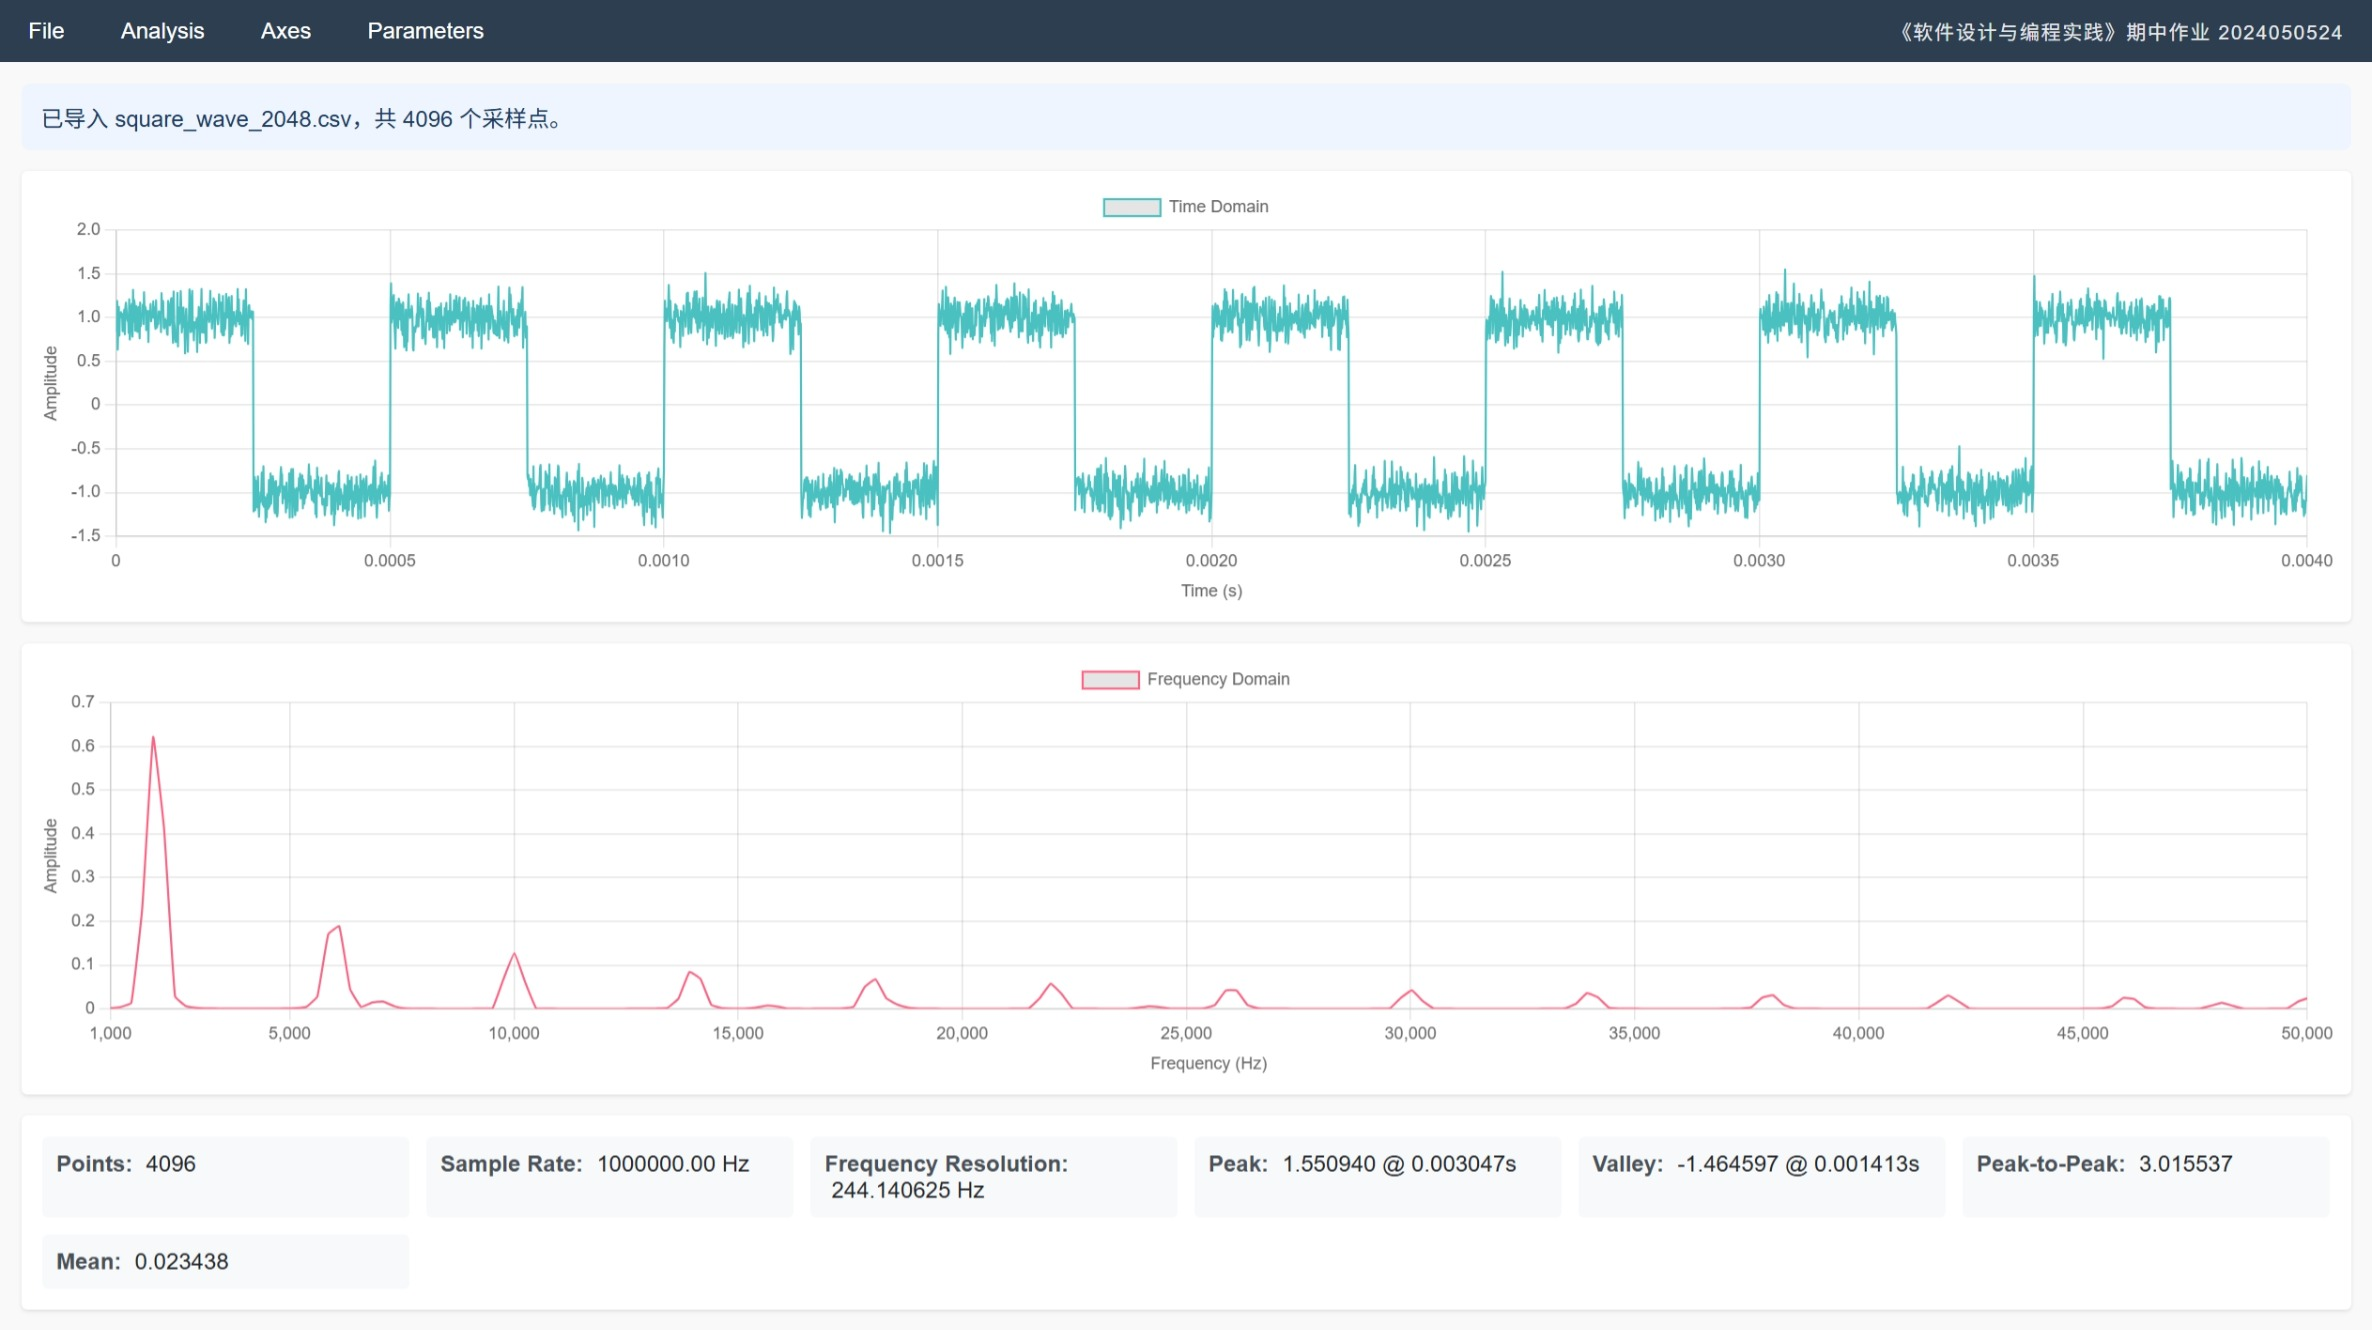
\includegraphics[width=0.82\textwidth]{image/4-21-3.jpeg}
  \caption{方波信号测试结果}
\end{figure}

\begin{figure}[H]
  \centering
  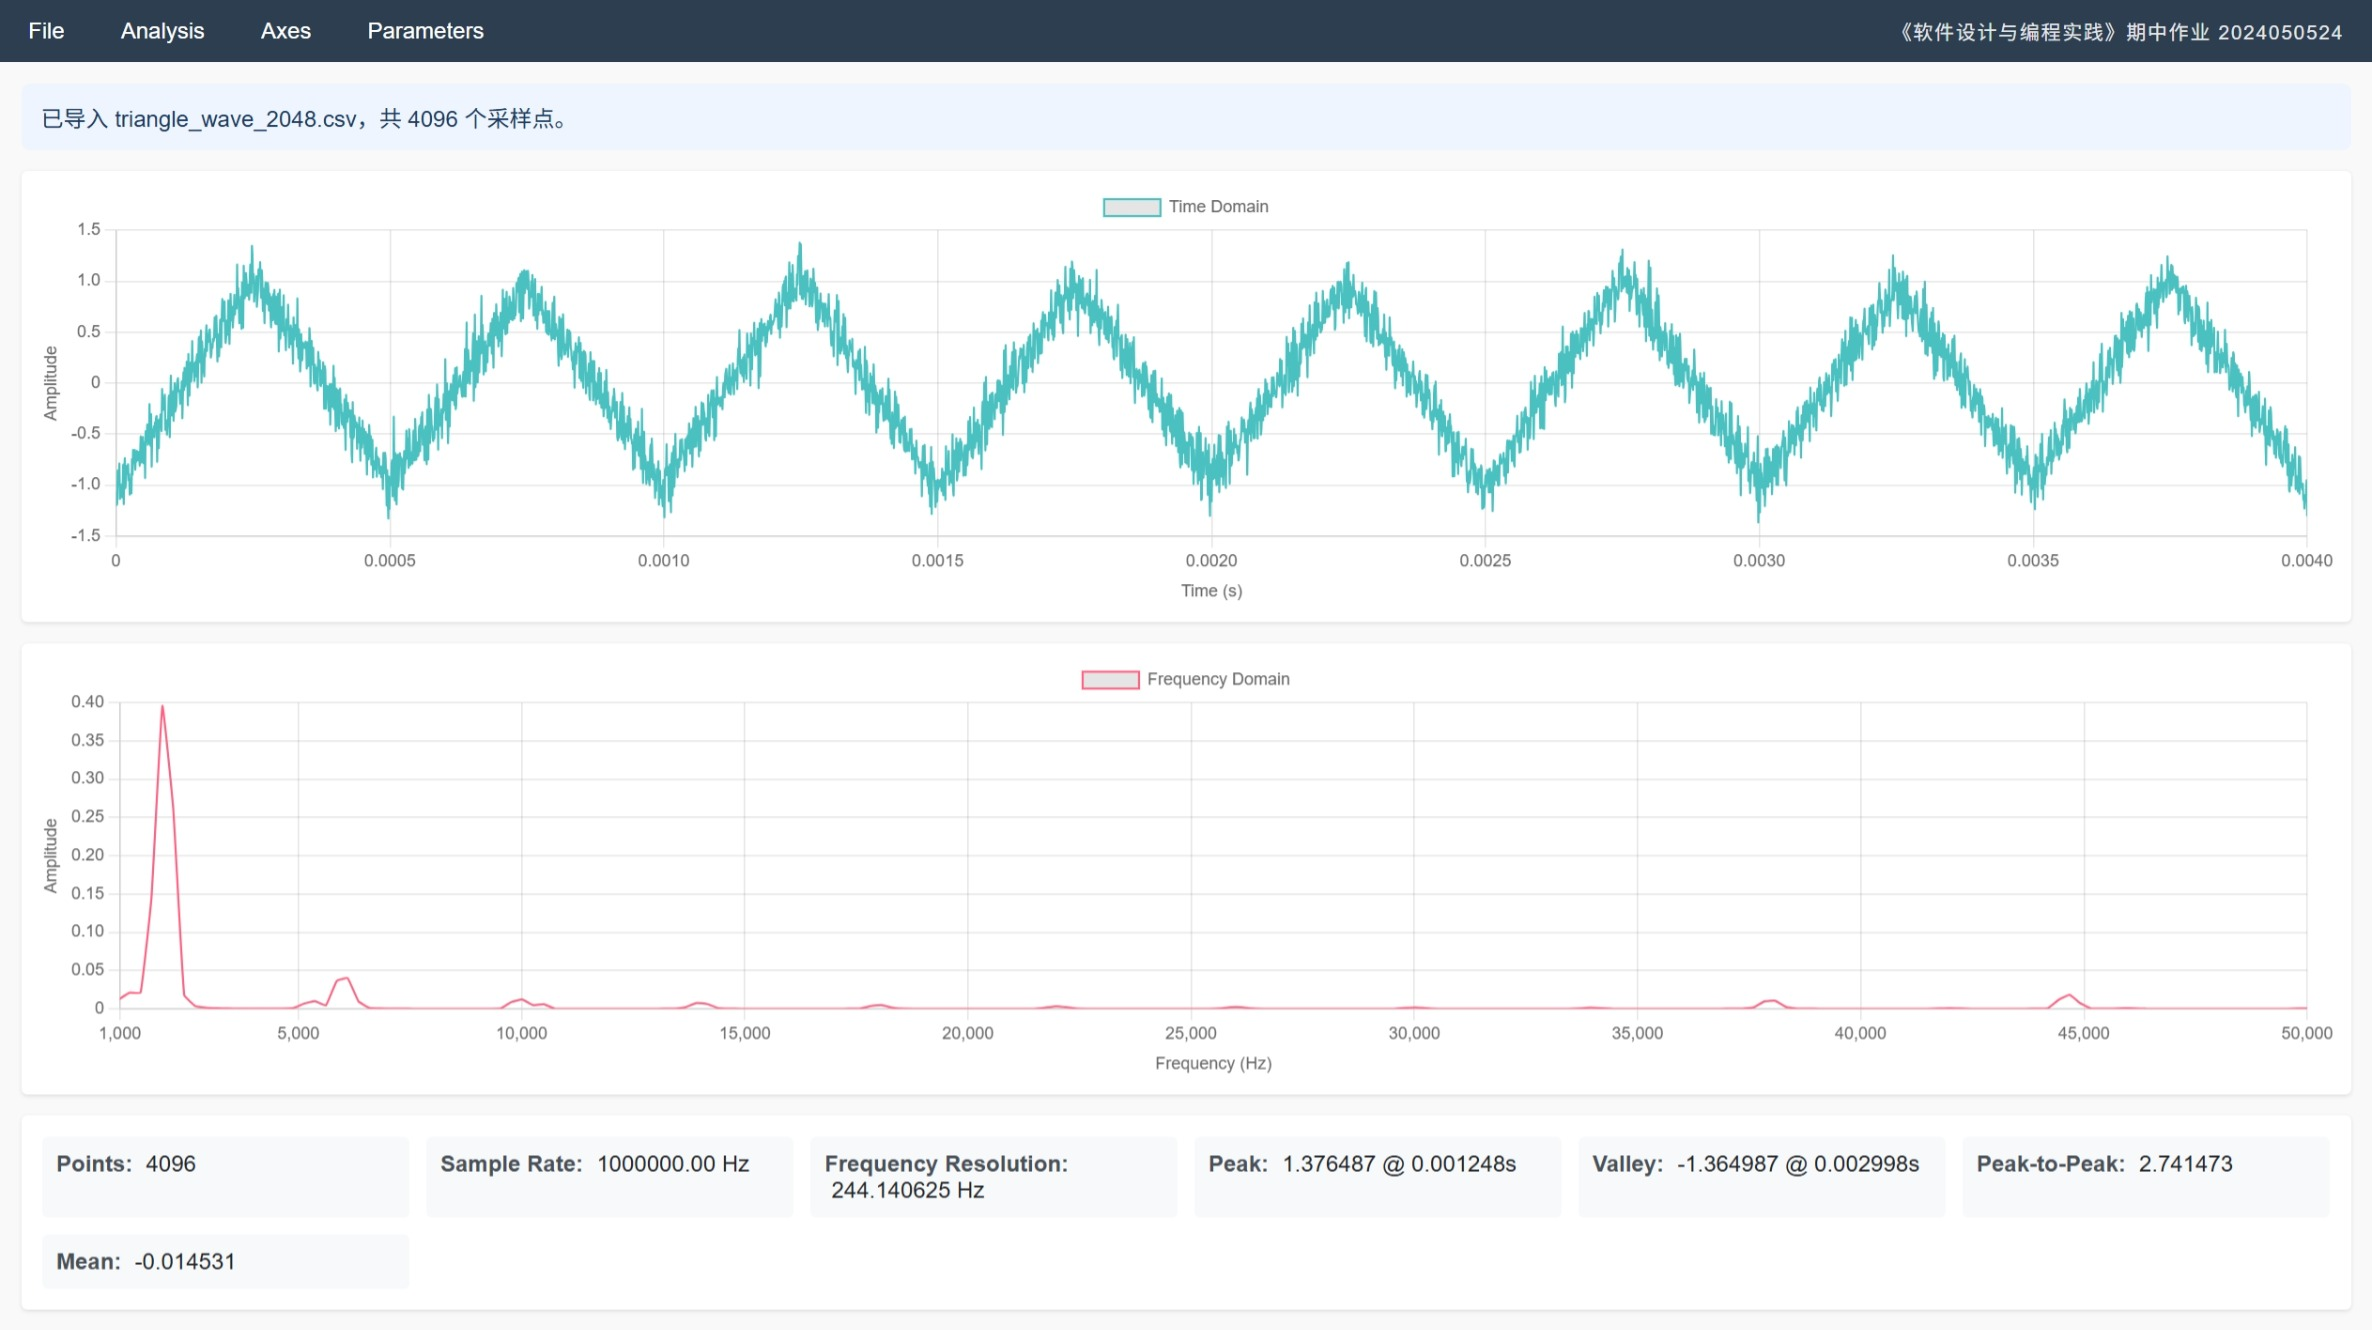
\includegraphics[width=0.82\textwidth]{image/4-21-4.jpeg}
  \caption{三角波信号测试结果}
\end{figure}

\begin{itemize}
  \item \textbf{方波信号}：用于验证时域分析模块对非正弦波形的处理能力。
  \item \textbf{三角波信号}：用于测试频域分析模块对不同波形的频率成分提取能力。
\end{itemize}

\section{实验总结}

本次实验完成了基于 Web 的交互式信号时域与频域分析工具开发。通过本次实验，验证了数字信号处理中时域分析与频域分析的基本原理，掌握了快速傅里叶变换（FFT）算法的实现及应用，同时也加强了对前端 Web 技术在数据处理与可视化方面应用的理解。

通过本次实验，可以得到以下结论：

\begin{enumerate}
  \item \textbf{算法层面}：时域分析能够直接展示信号幅值随时间的变化，频域分析能够清晰提取信号的频率组成，两者结合可以全面描述信号特征；FFT 算法能够高效完成时频域转换，适用于大规模采样数据处理。
  \item \textbf{编程方法层面}：通过模块化设计，将程序划分为初始化、数据导入、信号分析和可视化等独立模块，有助于降低耦合度、提升可维护性与可扩展性；事件驱动模型也很好地适配了 Web 端交互场景。
  \item \textbf{测试方法层面}：使用带噪声的实际测试信号对程序进行了较全面的验证，覆盖了数据导入、时域分析、频域分析和交互功能等多个方面，并通过与理论结果对比验证了程序正确性。
\end{enumerate}

本次实验实现的工具可直接用于 CSV 格式采样信号的快速分析，用户仅需通过浏览器即可完成操作，无需安装复杂专业软件，具有较强的实用价值。

\end{document}
